\chapter{Introduction}
\label{Introduction}
% learning a representation is important in ML:
There are many machine learning tasks in which the crux of the problem is in acquiring a representation for data such that meaningful features or relationships are easily read-out and exploited. E.g., the ubiquitous ML task of classification can be solved by looking at the nearest labeled neighbor, given that one had the proper metric in the first place. 
Another example is the task of information retrieval, which given the proper metric can be reduced as well to nearest neighbor queries.

% especially when high-level semantics are involved:
In tasks related to machine understanding of high-level semantics, the ability to learn a meaningful data representation is especially important since data is usually given in "low-level" terms (e.g. pixel intensities in digital images, audiograms for sound recordings, etc.) from which high-level concepts cannot be naively decoded, since individual features do not correlate with labels, and complex combinations of them need to be considered. \\
% undone 
E.g. while for data such as the MNIST handwritten-digit classification dataset, fitting a naive logistic regression model yields a classifier with a test accuracy of $92\%$, %\cite{tf tutorial}
while attempting to do so for the real-world image dataset CIFAR10 results in a test accuracy of only $33.5\%$. %\cite{stanford cs 299 hw}
Similarly, fitting a Gaussian kernel regression model on MNIST yields  test accuracy, while doing the same for CIFAR10 results only in a test accuracy of $54\%$. Both these models predict a class label by relying on direct weighting of features, which in this case were simply the low-level pixel intensities. 

\bigskip
\begin{table}[h!]
\centering
\noindent
\resizebox{20em}{!}{%
\begin{tabular}{|l||*{2}{c|}}\hline
\backslashbox{Model}{Dataset}
&\makebox[4em]{MNIST}&\makebox[4em]{CIFAR10}\\\hline\hline
Logistic Regression &$92\%$&$33.5\%$\\\hline 
Gaussian Kernel Regression &$98.7\%$&$54\%$\\\hline
\end{tabular}%
}
\caption{\label{tab:naive_features} Test accuracy for some common models using naïve features}
\end{table}
Arguably, natural cognitive agents in the wild also do not represent image or sound observations merely as arrays of floating point numbers.
\begin{figure}
\centering
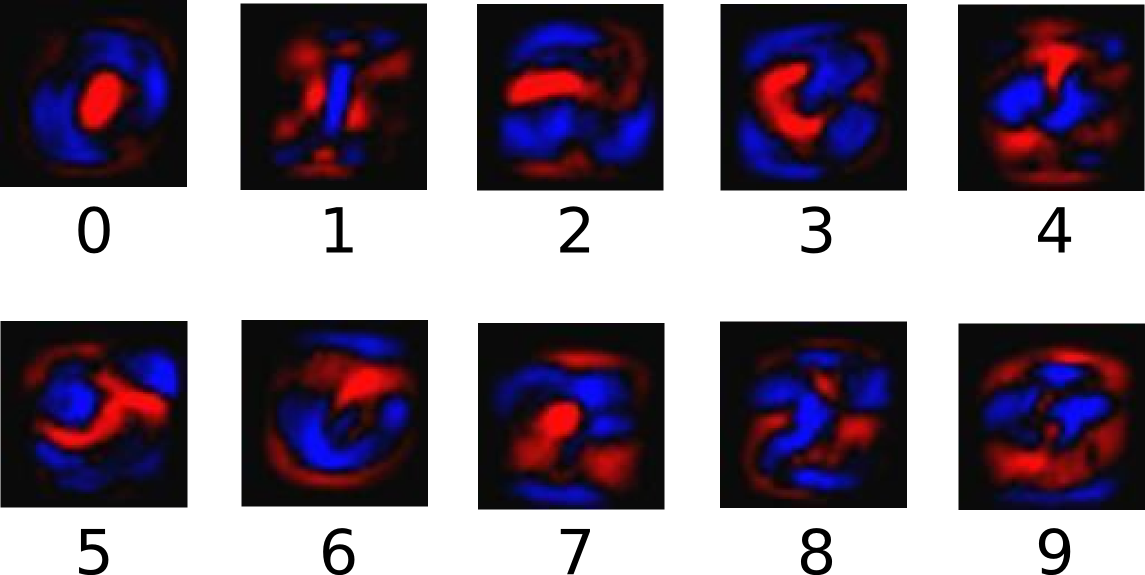
\includegraphics[width=0.6\textwidth]{imgs/softmax-weights.png}
\caption{\label{fig:softmax-weights}  Weights learned by a fitting a logistic regression model on the MNIST dataset. Red represents negative weights, while blue represents positive weights. The Logistic Regression model learns correlation between individual features and labels.}
\end{figure}

% private case: learning a similarity notion for cluster analysis
As a private case, in the task of cluster analysis, clustering algorithms search for clusters with regard to some similarity notion. The meaningfulness of these algorithms' outputs resides on whether the underlying similarity notion was meaningful in the first place.

%Representation of similarity notion. metric learning
A common approach to represent a similarity notion, which we also take in this work, is to 
% applications regardles of cluster analysis

---------------------> HERE
What metric would be applicable for real world images?
In real-world image semantics, 
it is crucial to have a meaningful, high-level similarity notion, since 
E.g. applying standard metrics (such as the Euclidean metric, Minkowski metrics, etc.) will fail to capture semantic similarity on real-world data.

% our problem setting
To formalize "meaningful", an ill-defined term, we focus in this work on transfer learning setups, where we attempt to learn a similarity notion under which clustering patterns conform best to a ground-truth desired clustering. The learned similarity notion will then be tested over data from different distibutions, which share the same underlying semantic similarity.  

% notation 
More formaly, we represent a clustering for $n$ data points $\{x_i\}_{i=1}^{n}$ from a data domain $\mathcal{D}$ as a boolean matrix $Y\in\{0,1\}^{n,n}$, where the $ij$'th entry is the indicator for whether $x_i$ and $x_j$ belong to the same cluster. 

% add image?

E.g most image understanding tasks are usually tackled today by first feeding the image to a neural network which ex  
For example in classification, if data can be represented as linearily seperated vector sets, then  

E.g image classification was trivial if the class identity  
Another example is in machine learning applications for games such as Chess or Go, where the learning system doesn't lea 


This is most relevant in domains where discrepency between low-level and high-level description is stark.
Computer vision is an example . low-level details need to be integrated 

In the task of cluster analysis for example, (it is done w.r.t representation)

There are many scenarios in which one needs to learn a representation for it's input
We focus on the case of clustering
natural to represent data as points in a metric space
we want to learn an embedding
Learning a joint embedding (deepsets)


% Explain Cluster Analysis: problem and motivation
% Explain Representation Learning: problem and motivation
% Private case: Metric Learning
% explain our pipeline embed,cluster,update. how we represent clustering (matrices)
% explain our contribution

\iffalse
In this work, we study the performance of end-to-end differentiable clustering algorithms.
The focus we shall take is on algorithms which can be factored to two processing steps:\\
a) Given an input set of data points, output an intermediate representation for them.\\
b) Given a set of data points under the new representation, apply a clustering algorithm over them.\\
This work focuses on the case where the entire processing is a differentiable function over a set of learnable parameters.\\
We will explore mainly the setting where the first step of the processing is done independently for each data-point, by embedding inputs $x_1,...,x_n$ to $f(x_1),...,f(x_n)$ for some function $f$.\\ We will also explore cases where this step is done "holistically", and the output representations of the different data points are co-dependent. \\  


(Arguably, an intelligent cognitive agent in the wild also does not store images as vectors of pixel intensities, sounds as audiograms, etc.) 
interpoint distances become less informative in high-dimensional spaces.


\section{Setup, notation, and definitions}
We consider the supervised learning problem of learning a clustering rule.\\ % change clustering rule to data representation or something like that..?
At each iteration of the learning process, the learner is presented with an ordered pair $<X,Y>$, consisting of $X\in\R^{nxd}$, a batch of $d$-dimensional data-points, and $Y\in {0,1}^{nxn}$, an $nxn$ binary matrix, whose $ij$'th entry indicates whether the $i$'th and $j$'th data points belong to the same cluster. The learner then outputs a soft clustering matrix $Y'\in [0,1]^{nxn}$ for which a loss of $L(Y,Y')$ is incurred, where $L$ is a loss function to measure the difference between the ground truth clustering and the predicted soft clustering.\\
We focus on the setting where the learner can bee seen as composed of two modules: \\
\begin{enumerate}
\item An embedding function $Emb_{\Theta}:\R^{nxd}\rightarrow\R^{nxd'}$, parameterized by $\Theta$, which maps the input batch $X$ to a representation $X'$.\\This could be implemented, for example, by a function which maps each data point $x_i\in X$ to $f_\Theta(x_i)$, where $f_\Theta$ belongs to some domain-relevant function space. At training, we update the parameters $\Theta$ in order to minimize $L(Y',Y)$. 
\item A clustering function $Clst:\R^{nxd'}\rightarrow [0,1]^{nxn}$ which is not parametrized, and therefor kept fixed throughout the learning process.
\end{enumerate}
The motivation for focusing on this specific decomposition is that the hollistic module includes interaction-wise parameters, and thus for better generalization and easier training, we would like to have this module fixed.\\ We Later explore some other decompositions, e.g those with learnable hollistic modules. \\
Theoretical question:\\
Learning optimal 1-d projection via gradient descent, in the case of two gaussians. Does the loss surface has good geometric properties?
 If the data is adversarialy generated, is the problem NP hard?
\subsection{Definitions}
For every set X of size n, we can represent a clustering over that set as an nxn matrix Y, whose ij'th entry 0/1 indicating whether the i'th and j'th elements share the same cluster.
  An equivalent way to represent a clustering, which assumes an underlying indexing for the different clusters, is to represent it by a nxk membership matrix B, for which the ij'th entry is 0/1 whether the i'th element is a member of the j'th cluster.\\
 \subsection{Mathematical properties of clustering matrices}
 $\ B B^T=Y$\\
 The ground truth matrix is a rank $k$ projection matrix.
 The normalizing matrix who's diagonals are the cluster sizes is $\ B^T B=Y$
 The Centroid matrix is the penrose-moore inverse of the assignment matrix, times the data matrix \cite{banarjee05}.\\ 
\fi